\chapter{Klasyczne metody detekcji ruchu na scenie}
\label{cha:metodyStare}
%\section{Średnia bieżąca}
%Algorytm średniej bieżącej to bezparametrowa metoda detekcji ruchu oparta na zależnościach statystycznych. Polega ona na analizie rozkładu prawdopodobieństwa wystąpienia pewnych wartości jasności (koloru) piksela na podstawie jego sąsiedztwa.\\
%\nocite{kheng2011mean}
%Średnia bieżąca (ang. \textit{mean shift}) wyznaczana jest metodą iteracyjną dla każdej próbki obrazu oddzielnie. Dla danego piksela x oblicza się średnią tymczasową m(x) z jego otoczenia, która przedstawia się wzorem:
%\begin{equation}
%m(x) = 
%\frac{\sum_{i=1}^{n}K(x-x_{i})x_{i}}{\sum_{i=1}^{n}K(x-x_{i})}
%\end{equation}
%, gdzie K - kernel, w którym zawarte są wagi, z jakimi brane są pod uwagę piksele sąsiedztwa x\textsubscript{i}, n - ilość pikseli sąsiedztwa \\
%Średnią bieżącą nazywamy różnicę m(x) - x.
%Następnie należy sprawdzić, czy wartość piksela równa jest średniej tymczasowej, czyli czy m(x) == x. Jeśli nie - należy przypisać x = m(x) i rozpocząć wyznaczanie średniej dla nowej wartości x. Jeśli jednak tak, algorytm kończy się.\\
%Jeśli średnie tymczasowe obliczane są dla wielu punktów, aktualizacja ich wartości odbywa się równocześnie w każdej iteracji.
%\paragraph{}
%W ten sposób otrzymana średnia bieżąca może zostać użyta do wykrywania ruchu na scenie. Tworzona jest mapa gęstości prawdopodobieństwa na podstawie histogramu kolorów obiektu w poprzedniej ramce (dla każdego piksela osobno), a następnie wyszukuje się w niej szczytowej wartości w pobliżu wcześniejszego położenia obiektu. Pozwala to na wykrycie kierunku ruchu obiektu zmieniającego położenie.
%\paragraph{}
%Najczęściej wspominaną wadą takiego podejścia jest konieczność używania stałej wielkości ramki, w której ma znajdować się śledzony obiekt. Niewygodne staje się więc śledzenie obiektów zmieniających rozmiar w czasie, jak np. nadjeżdżających samochodów obserwowanych z odpowiedniej perspektywy. Bardziej elastyczną wersją tej metody jest CAMSHIFT (ang. \textit{Continuous Adaptive Mean Shift}, potrafiąca dostosować się do zmian w kolorystyce obiektu, a także jego rozmiarze. Implementacja obu algorytmów dostępna jest w bibliotece OpenCV.

\section{Gaussian Mixture Model}
\label{sec:GMM}
Metoda ta \cite{zivkovic2004improved} opiera się na obserwacji, iż obiekty tła, przy braku przemieszczających się obiektów na scenie, wykazują pewne zależności, które mogą zostać przedstawione za pomocą modeli statystycznych. Dlatego też wyodrębnienie pikseli nie pasujących do takiego modelu wiąże się z wykryciem ruchu na scenie. Jest to stosunkowo mało skomplikowany algorytm oparty na mechanizmie subtrakcji tła.
\paragraph{}
Pierwszym etapem działania algorytmu jest wyznaczenie modelu tła. Odbywa się to na podstawie gaussowskiego rozkładu prawdopodobieństwa dla każdego piksela sceny. Estymowane wartości modelu tła otrzymywane są w wyniku analizy określonej liczby próbek w czasie t. Następnie odbywa się klasyfikacja pikseli. Jeżeli prawdopodobieństwo wystąpienia danego piksela w ramce t+n jest większe od pewnego ustalonego progu, zostaje on sklasyfikowany jako tło. W przeciwnym wypadku przypisuje się go do modelu pierwszoplanowego.\\
Głównym problemem, z jakim spotyka się ta metoda, jest problem z adaptacją do zmian na scenie, na przykład w oświetleniu.\\
Prawdopodobieństwo wystąpienia danej wartości piksela $x$ (z uwzględnieniem jasności na wszystkich kanałach) w ramce $t$ przy $K$ jako liczbie gausjanów używanych w modelu z wagą $w$ dane jest następującym wzorem:
\begin{equation}
P(x_{t}) = \sum_{i=1}^{K} w_{i,t}*g(x_{t},\mu_{i,t},\Sigma_{i,t})
\end{equation}
przy czym funkcja gęstości prawdopodobieństwa dla rozkładu Gaussa:
\begin{equation}
g(x,\mu,\Sigma) = \frac{1}{\sqrt{|\Sigma|}\sqrt{2\pi}}\mathrm{e}^\frac{-(x-\mu)^T\Sigma^{-1}(x-\mu)}{2}
\end{equation}
gdzie:\\ 
\hspace*{3em}
\begin{tabular}{r l}
$\mu$: & wartość średnia \\
$\Sigma$: & macierz kowariancji
\end{tabular} \\

Macierz kowariancji dla uproszczenia traktowana jest jako iloczyn kwadratu odchylenia standardowego i macierzy jednostkowej:
\begin{equation}
\Sigma_{k,t}=\sigma_{k,t}^2I
\end{equation}
Takie podejście umożliwia stworzenie multomodalnej reprezentacji tła, co jest szczególnie ważne dla segmentacji w obecności drobnego ruchu na scenie - piksele ruchomych fragmentów tła mogą przyjmować wtedy skrajne wartości w czasie, reprezentowanie ich więc w modelu referencyjnym poprzez pojedyncze liczby często prowadzi do poważnych błędów w działaniu algorytmu. \\ 
Głównym zagadnieniem dla tej metody jest kwestia doboru próbek, na podstawie których wyznaczane jest prawdopodobieństwo. Zbyt mała bądź źle dobrana ich ilość powoduje fałszywą detekcję w przypadku znacznej zmienności tła, zbyt duża - zawyżoną tolerancję, przez co piksele pierwszoplanowe zostają niekiedy sklasyfikowane jako tło. Próg tolerancji również musi się różnić w zależności od poziomu jasności pikseli, ponieważ w zacienionych obszarach z reguły dużo rzadziej występuje zaszumienie.
\subsection{Uaktualnianie modelu tła}
Jak wspomniano, do poprawnej detekcji w dłuższych przedziałach czasowych niezbędne jest ciągłe uaktualnianie modelu tła. Z tego też powodu odpowiednie wartości uaktualniane są zgodnie z następującymi wzorami:
\begin{gather}
w_{k,t} = w_{k,t-1}+\alpha(o_{k,t}-w_{k,t-1}) \\
\mu_{k,t} = \mu_{k,t-1}+o_{k,t}\frac{\alpha (x_{t}-\mu_{k,t-1})}{w_{k,t}} \\
\sigma^2_{k,t} = \sigma^2_{k,t-1}+o_{k,t}\frac{\alpha ((x_{t}-\mu_{k,t})^{T}(x_{t}-\mu_{k,t})-\sigma^2_{k,t-1})}{w_{k,t}}
\end{gather}
gdzie:\\ 
\hspace*{3em}
\begin{tabular}{r l}
$\alpha$: &  parametr ''uczący'' \\
$o$: & binarna wartość ustalana na 1 dla najbliższego komponentu spośród modeli $K$
\end{tabular} \\

Jeśli nie znaleziono wystarczająco bliskiego komponentu (odległego o mniej niż ustalony próg), nowy komponent tworzony jest z parametrami $w_{K+1,t} = \alpha, \mu{K+1,t}= x_{t}, \sigma_{K+1,t}=\sigma_{0}$. Jeśli nastąpi przepełnienie bufora komponentów, ten z najmniejszą wagą jest odrzucany. 
\paragraph{}
Opisywana metoda dostępna jest w bibliotece OpenCV w postaci klasy \textit{BackgroundSuntractorMog2}. Choć daje ona stosunkowo dobre wyniki przy statycznym tła, drobny ruch sceny powoduje wzrost liczby fałszywych detekcji. Przykład takiego zjawiska przedstawiony jest na rys. \ref{fig:GMM}.

\begin{figure}[!h]
\centering
\begin{subfigure}[b]{0.4\textwidth}
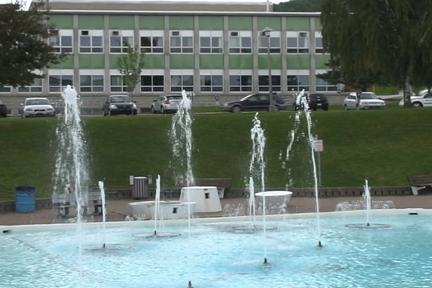
\includegraphics[width=\textwidth]{img/GMMIn}
\caption{}
\end{subfigure}
\quad
\begin{subfigure}[b]{0.4\textwidth}
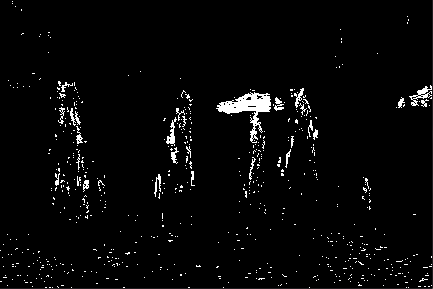
\includegraphics[width=\textwidth]{img/GMMOut}
\caption{}
\end{subfigure}
\caption{Wynik dla ramki numer 712 z zestawu \textit{fountain01}. (a) - oryginalny obraz, (b) - rezultat segmentacji.\label{fig:GMM}}
\end{figure}


\section{ViBE}
Autorzy pracy \cite{barnich2011vibe} zaproponowali jeszcze inny sposób na dokonywanie segmentacji obiektów pierwszoplanowych w zmieniających się warunkach otoczenia. Zamiast modelować i przewidywać wartość piksela, postanowili oni przechowywać informację o jego wcześniejszych reprezentacjach.
\paragraph{}
ViBE (ang. \textit{VIsual Background Extractor}) porzuca koncepcję estymacji pożądanej wartości piksela na podstawie wielu próbek, mogących zawierać informacje skrajnie odbiegające od średnich. Zamiast tego skupia się na badaniu podobieństwa aktualnego piksela do jego reprezentacji zarejestrowanych uprzednio - przechowywanie informacji o jego historii pozwala lepiej radzić sobie w warunkach drobnego ruchu na scenie.
\subsection{Opis metody}
Niech piksel $x$, którego wartość w przestrzeni barwnej oznaczona jest jako $v(x)$, reprezentowany jest w czasie jako zbiór poprzednich wartości $v_{i}$:
\begin{equation}
\label{eq:prevValVibe}
M(x) = \left\{v_{1}, v_{2}, ..., v_{n}\right\}
\end{equation}
Klasyfikacja $x$ odbywa się poprzez zbadanie odległości $v(x)$ od każdego elementu ze zbioru $M(x)$. Jeśli jest ona mniejsza od pewnego ustalonego progu ($v(x)$ i $v_{k}$ są odpowiednio bliskie), następuje zwiększenie licznika odpowiadającego pewnemu stopniowi podobieństwa badanego piksela do swojej historii. Po przekroczeniu pewnego progu podobieństwa piksel klasyfikowany jest jako tło, dalsze sprawdzanie odległości można pominąć.
\paragraph{Inicjalizacja modelu tła \\}
W odróżnieniu od wielu innych metod, uczących się na sekwencji testowej, inicjalizacja tła w algorytmie ViBE może odbywać się na podstawie pojedynczej ramki. Umożliwia to nie tylko szybki start faktycznej detekcji, ale także błyskawiczną adaptację do nagłych zmian oświetlenia na scenie. Ponieważ w pojedynczej ramce nie są zawarte żadne informacje na temat zachowania piksela w czasie, budowanie wzorca odbywa się na podstawie jego sąsiedztwa i wynika z założenia, że ich dystrybucje czasowe są podobne. Z tego też powodu dla piksela $x$ zbiór $M(x)$ (równanie \ref{eq:prevValVibe}) wypełniany jest losowo wybranymi wartościami z jego otoczenia. W zależności od rozmiaru sąsiedztwa i liczności zbioru $M$ niektóre wartości mogą zostać wylosowane wielokrotnie.\\
Ryzykiem towarzyszącym takiemu podejściu jest możliwość powstawania wspomnianych już 'duchów' - jeśli w próbkowanej ramce znajduje się choćby fragment obiektu pierwszoplanowego, sklasyfikowany zostaje on błędnie jako tło. Z tego powodu odsłonięty w kolejnych ramkach prawdziwy dalszy plan wykrywany jest jako obiekt poruszający się. Z tym zjawiskiem radzi sobie jednak mechanizm uaktualniania tła.
\paragraph{Utrzymywanie modelu \\}
Jak wspomniano, raptowne zmiany oświetlenia i artefakty pozostałe po błędnej klasyfikacji mogą zaburzać proces detekcji. Aby uniezależnić się od tych czynników, autorzy rozwiązania zaproponowali proces uaktualniania modelu tła polegający na zamianie wartości referencyjnych modelu aktualnie zakwalifikowanymi jako tło. W odróżnieniu jednak od podejść stosowanych w innych algorytmach, polegających na pozbywaniu się wartości najstarszych bądź z wykorzystaniem informacji o częstości występowania (wadze) reprezentacji piksela w przeszłości, postanowili użyć metody losowej, biorącej pod uwagę funkcję gęstości prawdopodobieństwa. Zmodyfikowali więc metodę konserwatywnej aktualizacji modelu tła w taki sposób, aby dodatkowo wykorzystywała informację o sąsiedztwie. Ponadto, aktualizacja tła nie odbywa się dla każdego piksela co ramkę - przy klasyfikacji dokonywana jest losowa decyzja, czy dana wartość ma zastąpić starą próbkę. Ponieważ używana jest metoda konserwatywna, w\,celu pozbycia się ryzyka propagacji błędnej klasyfikacji od czasu do czasu aktualizacja tła odbywa się na podstawie sąsiednich pikseli, jak opisano w sekcji dotyczącej inicjalizacji tła. Wynik detekcji przedstawiony został na rys. \ref{fig:ViBE} 
\begin{figure}[!h]
\centering
\begin{subfigure}[b]{0.4\textwidth}
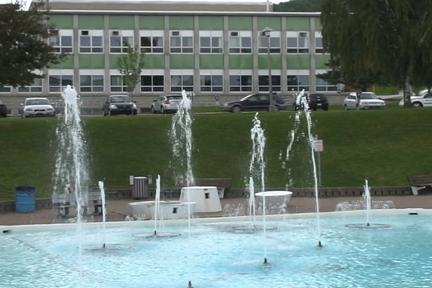
\includegraphics[width=\textwidth]{img/GMMIn}
\caption{}
\end{subfigure}
\quad
\begin{subfigure}[b]{0.4\textwidth}
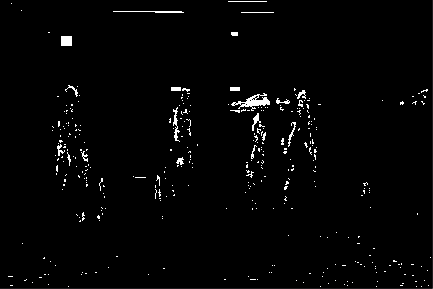
\includegraphics[width=\textwidth]{img/ViBEOut}
\caption{}
\end{subfigure}
\caption{Wynik dla ramki numer 712 z zestawu \textit{fountain01}. (a) - oryginalny obraz, (b) - rezultat segmentacji.\label{fig:ViBE}}
\end{figure}


\section{PBAS}
Podobnie jak w przypadku algorytmu ViBE, autorzy metody PBAS proponują modelowanie tła przy pomocy zbioru poprzednich wartości piksela z losową ich aktualizacją. Podstawową różnicą jest jednak traktowanie parametrów aktualizacji jako zmiennych, dostosowujących się w czasie do wartości każdego z pikseli osobno. Opisywana w artykule \cite{hofmann2012background} metoda opiera się na klasyfikacji piksela na podstawie modelu tła $B$ w zależności od macierzy progów $R$. Uaktualnianie modelu w czasie odbywa się przy pomocy dostosowującego się w czasie i indywidualnego dla każdego piksela parametru $T$. Jak ukazano na rys. \ref{fig:PBAS}, wydaje się to najlepszym rozwiązaniem dla scen o dynamicznym tle.
\subsection{Segmentacja}
W przypadku tej metody decyzja o tym, czy piksel $x$ należy do tła, odbywa się poprzez porównanie jego wartości z uprzednio zarejestrowanymi. Jeśli $I(x)$ (aktualnie analizowana wartość piksela) różni się od porównywanego modelu tła $B(x)$ o mniej, niż próg $R(x)$ dla przynajmniej $\#_{min}$ próbek, zostaje on zaklasyfikowany jako tło, w przeciwnym wypadku uznaje się, iż należy do pierwszego planu.
\subsection{Uaktualnianie modelu tła}
Uaktualnianie modelu tła odbywa się zgodnie z metodą konserwatywną. Ponieważ w modelu znajduje się $N$ poprzednich próbek dla piksela, losowo wybrana z nich $x_{k}$ zostaje zastąpiona przez aktualnie pobraną jego wartość. Nie odbywa się to jednak każdorazowo - wybrany element ze zbioru jest podmieniany z prawdopodobieństwem $p = 1/T(x)$, czyli zależnie od parametru zawartego w macierzy aktualizacji. Dodatkowo dla modelu, z którego wybrana została próbka ($B_{k}$), dokonywana jest z takim samym prawdopodobieństwem aktualizacja losowo wybranego piksela z sąsiedztwa $x_{k}$ jego wartością z ramki analizowanej.
\paragraph{}
Jak wspomniano, aktualizowane są tylko piksele zakwalifikowane jako tło. Modyfikacja modelu sąsiedztwa piksela odbywa się jednak bez sprawdzania żadnych warunków - oznacza to, iż może on zostać zmieniony pomimo przynależności wybranego piksela do modelu pierwszoplanowego. Powoduje to zmniejszenie czasu propagacji fałszywych detekcji oraz zanikanie obiektów zatrzymanych.
\subsection{Dostosowywanie macierzy parametrów}
W celu poprawnego działania algorytmu zarówno macierz progów $R$, jak i stopnia uczenia się $T$ muszą dostosowywać się do zmiennych warunków na scenie. Pozwala to uniknąć błędnych detekcji, zwłaszcza w przypadku dynamicznego ruchu tła.\\
Przy aktualizacji macierzy $R$ wykorzystywane są informacje zawarte w pomocniczej tablicy macierzy odległości $D$. Modyfikowana jest ona przy każdorazowej aktualizacji modelu tła $B_{k}(x)$ jako minimalna odległość między wartością piksela a jego odpowiednikiem w modelu referencyjnym:
\begin{equation}
D_{k}(x)=min_{k}dist(I(x),B_{k}(x))
\end{equation}
Średnia wartość $\bar{d}_{min}(x)$ tak obliczonych współczynników dla każdego piksela odpowiada stopniowi dynamiki tła w danym punkcie. Macierz $R$ uaktualniana jest więc według poniższego równania:
\begin{equation}
R(x) = \left\{
\begin{split}
&R(x)(1-R_{inc/dec}) & \quad &\text{dla $R(x)>\bar{d}_{min}(x)\cdot R_{scale}$} \\
&R(x)(1+R_{inc/dec}) & \quad &\text{w przeciwnym wypadku}
\end{split}
\right.
\end{equation}
gdzie:\\ 
\hspace*{3em}
\begin{tabular}{r l}
$R_{inc/dec}$: &  stała przyrostu/spadku wartości macierzy\\
$R_{scale}$: & stała skala podobieństwa
\end{tabular} \\

Ponieważ poprawność detekcji w dużej mierze zależy od dynamiki tła, parametr $\bar{d}_{min}$ wykorzystywany jest również w przypadku aktualizacji macierzy $T$, od której zależy prawdopodobieństwo aktualizacji modelu tła:
\begin{equation}
T(x) = \left\{
\begin{split}
&T(x)+\frac{T_{inc}}{\bar{d}_{min}(x)} & \quad &\text{jeśli $x$ należy do pierwszego planu} \\
&T(x)-\frac{T_{dec}}{\bar{d}_{min}(x)}) & \quad &\text{w przeciwnym wypadku}
\end{split}
\right.
\end{equation}
gdzie:\\ 
\hspace*{3em}
\begin{tabular}{r l}
$T_{inc}$: &  stała przyrostu prawdopodobieństwa\\
$T_{dec}$: & stała spadku prawdopodobieństwa
\end{tabular} \\

\paragraph{}
W celu likwidacji zakłóceń powstałych w wyniku fałszywych detekcji dla zaszumionych obszarów i drobnych niedoskonałości klasyfikacji, wyniki poddawane są dodatkowo filtracji medianowej.

\begin{figure}[!h]
\centering
\begin{subfigure}[b]{0.4\textwidth}
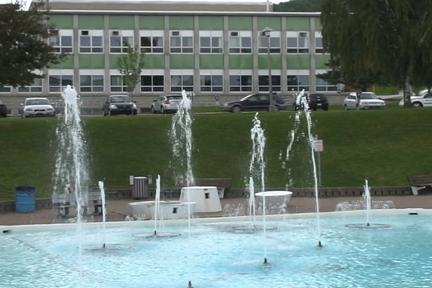
\includegraphics[width=\textwidth]{img/GMMIn}
\caption{}
\end{subfigure}
\quad
\begin{subfigure}[b]{0.4\textwidth}
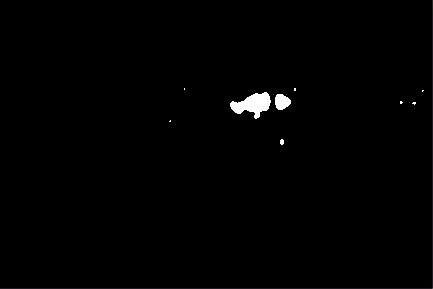
\includegraphics[width=\textwidth]{img/PBASOut}
\caption{}
\end{subfigure}
\caption{Wynik dla ramki numer 712 z zestawu \textit{fountain01}. (a) - oryginalny obraz, (b) - rezultat segmentacji.\label{fig:PBAS}}
\end{figure}